\chapter{Galvanic Cells, Electrodes \& Electrochemical Series}
\label{chap:galvanic_cells}

\section{Origin of Electrode Potential \& The Electrical Double Layer}

When a strip of metal $\ce{M}$ is immersed into an aqueous solution containing its own ions $\ce{M^{z+}}$, two opposing dynamic processes immediately commence at the solid-liquid phase interface:

\begin{enumerate}[leftmargin=*]
    \item \textbf{De-electronation (Dissolution tendency):}
    Metal atoms on the surface tend to lose valence electrons to the metal lattice and pass into solution as hydrated cations:
    \begin{equation}
        \ce{M(s) -> M^{z+}(aq) + z e^-} \quad (\text{Oxidation})
    \end{equation}
    This tendency is governed by the \textbf{solution pressure} ($P$) of the metal (Nernst's electrolytic solution pressure theory). As positive ions enter the solution, a surplus of electrons is left behind on the metal surface, charging the electrode negatively relative to the solution.

    \item \textbf{Electronation (Deposition tendency):}
    Conversely, solvated cations $\ce{M^{z+}}$ in solution collide with the electrode surface, capture electrons from the metal, and deposit as neutral metal atoms:
    \begin{equation}
        \ce{M^{z+}(aq) + z e^- -> M(s)} \quad (\text{Reduction})
    \end{equation}
    This tendency is driven by the \textbf{osmotic pressure} ($p$) of the metal ions in solution. As electrons are extracted from the metal, the electrode acquires a positive charge relative to the solution.
\end{enumerate}

\begin{figure}[htbp]
\centering
\begin{tikzpicture}[scale=1.1]
    % (a) Negative Electrode: P > p
    \begin{scope}[shift={(0,0)}]
        \draw[thick] (0,0) rectangle (3.5,3);
        \fill[blue!8] (0.05,0.05) rectangle (3.45,2.4);
        \node[above] at (1.75,3.0) {\textbf{(a) $P > p$ (Anode)}};
        
        % Metal rod
        \draw[fill=gray!40, thick] (1.3,0.5) rectangle (2.2,3.5);
        \node at (1.75,2.0) {\small $\ce{Zn}$};
        
        % Negative charges on rod
        \foreach \y in {0.8, 1.2, 1.6, 2.4, 2.8} {
            \node[red, font=\bfseries] at (1.45,\y) {$-$};
            \node[red, font=\bfseries] at (2.05,\y) {$-$};
        }
        % Positive ions in solution
        \node[blue, font=\bfseries] at (0.8,1.2) {\footnotesize $\ce{Zn^2+}$};
        \node[blue, font=\bfseries] at (2.7,1.2) {\footnotesize $\ce{Zn^2+}$};
        \node[blue, font=\bfseries] at (0.8,2.0) {\footnotesize $\ce{Zn^2+}$};
        \node[blue, font=\bfseries] at (2.7,2.0) {\footnotesize $\ce{Zn^2+}$};
        \draw[->, thick, blue] (1.3,1.2) -- (0.9,1.2);
        \draw[->, thick, blue] (2.2,1.2) -- (2.6,1.2);
        \node[below] at (1.75,-0.2) {\small Negative Potential ($\phi_M < \phi_S$)};
    \end{scope}

    % (b) Positive Electrode: p > P
    \begin{scope}[shift={(5.5,0)}]
        \draw[thick] (0,0) rectangle (3.5,3);
        \fill[blue!8] (0.05,0.05) rectangle (3.45,2.4);
        \node[above] at (1.75,3.0) {\textbf{(b) $p > P$ (Cathode)}};
        
        % Metal rod
        \draw[fill=orange!30, thick] (1.3,0.5) rectangle (2.2,3.5);
        \node at (1.75,2.0) {\small $\ce{Cu}$};
        
        % Positive charges on rod
        \foreach \y in {0.8, 1.2, 1.6, 2.4, 2.8} {
            \node[blue, font=\bfseries] at (1.45,\y) {$+$};
            \node[blue, font=\bfseries] at (2.05,\y) {$+$};
        }
        % Negative ions in solution
        \node[red, font=\bfseries] at (0.8,1.2) {\footnotesize $\ce{SO4^2-}$};
        \node[red, font=\bfseries] at (2.7,1.2) {\footnotesize $\ce{SO4^2-}$};
        \node[red, font=\bfseries] at (0.8,2.0) {\footnotesize $\ce{SO4^2-}$};
        \node[red, font=\bfseries] at (2.7,2.0) {\footnotesize $\ce{SO4^2-}$};
        \draw[->, thick, blue] (0.9,1.2) -- (1.3,1.2);
        \draw[->, thick, blue] (2.6,1.2) -- (2.2,1.2);
        \node[below] at (1.75,-0.2) {\small Positive Potential ($\phi_M > \phi_S$)};
    \end{scope}
    
    % (c) Stern Double Layer Model
    \begin{scope}[shift={(11,0)}]
        \draw[thick] (0,0) rectangle (3.8,3);
        \node[above] at (1.9,3.0) {\textbf{(c) Stern Double Layer}};
        \draw[fill=gray!40, thick] (0.2,0.2) rectangle (0.8,2.8);
        \node at (0.5,1.5) {\rotatebox{90}{\textbf{Electrode}}};
        \foreach \y in {0.5, 0.9, 1.3, 1.7, 2.1, 2.5} {
            \node[red, font=\bfseries] at (0.7,\y) {$-$};
        }
        % Helmholtz plane
        \draw[dashed, primarynavy] (1.4,0.2) -- (1.4,2.8);
        \foreach \y in {0.5, 0.9, 1.3, 1.7, 2.1, 2.5} {
            \node[blue, font=\bfseries] at (1.4,\y) {$+$};
        }
        % Diffuse layer
        \node[blue] at (2.2,0.7) {$+$};
        \node[red] at (2.5,1.2) {$-$};
        \node[blue] at (2.8,2.1) {$+$};
        \node[blue] at (3.2,1.5) {$+$};
        \node[red] at (3.4,0.8) {$-$};
        \node[below] at (1.4,0.1) {\scriptsize IHP/OHP};
        \node[below] at (2.7,0.1) {\scriptsize Diffuse Layer};
        \node[below] at (1.9,-0.2) {\small Helmholtz + Gouy-Chapman};
    \end{scope}
\end{tikzpicture}
\caption{Origin of Electrode Potential and the Electrical Double Layer structure.}
\label{fig:double_layer}
\end{figure}

At dynamic equilibrium, the rate of de-electronation equals the rate of electronation:
\begin{equation}
    \ce{M(s) <=> M^{z+}(aq) + z e^-}
\end{equation}
A separation of opposite electric charges is established across the interface over molecular dimensions ($\approx 1-10\text{ nm}$), forming the \textbf{electrical double layer}. 

\begin{conceptbox}[Definition of Electrode Potential]
The electric potential difference established between the metal electrode and the bulk electrolyte solution across the electrical double layer at dynamic equilibrium is termed the \textbf{Electrode Potential} ($E$):
\begin{equation}
    E = \phi_{\text{metal}} - \phi_{\text{solution}}
\end{equation}
\begin{itemize}[leftmargin=*]
    \item If $P > p$ (e.g., $\ce{Zn}$ in $\ce{ZnSO4}$), oxidation dominates initially, leaving excess electrons on the metal. The electrode is negatively charged relative to the solution ($E_{\text{ox}} > 0, E_{\text{red}} < 0$).
    \item If $p > P$ (e.g., $\ce{Cu}$ in $\ce{CuSO4}$), reduction dominates initially, consuming electrons from the metal. The electrode is positively charged relative to the solution ($E_{\text{red}} > 0, E_{\text{ox}} < 0$).
    \item When all participating chemical species are in their \textbf{thermodynamic standard states} (solute activities $a = 1\text{ M}$, gas fugacities $f = 1\text{ bar} \approx 1\text{ atm}$, pure solids/liquids, at $T = 298.15\text{ K}$), the potential difference is termed the \textbf{Standard Electrode Potential} ($E^\circ$).
\end{itemize}
\end{conceptbox}

\begin{atkinsbox}[Atkins Deep Dive: The Stern Model of the Electrochemical Double Layer]
According to Otto Stern (1924), the electrical double layer consists of two concentric zones:
\begin{enumerate}[leftmargin=*]
    \item \textbf{The Inner Helmholtz Plane (IHP):} The locus of electrical centers of specifically adsorbed, non-solvated ions on the electrode surface.
    \item \textbf{The Outer Helmholtz Plane (OHP):} The locus of centers of fully solvated counter-ions held purely by electrostatic forces at the distance of closest approach. The potential drops linearly between the metal surface and the OHP.
    \item \textbf{The Gouy-Chapman Diffuse Layer:} Beyond the OHP, thermal kinetic agitation prevents ions from forming a rigid sheet; instead, an exponentially decaying diffuse ionic atmosphere extends into the bulk solution. The potential drop across the diffuse shearing plane is the electrokinetic \textbf{Zeta Potential} ($\zeta$).
\end{enumerate}
\end{atkinsbox}

---

\section{Classification of Electrodes}

Electrodes employed in electrochemical cells and equilibrium studies are systematically classified into five major architectural categories:

\begin{table}[htbp]
\centering
\small
\renewcommand{\arraystretch}{1.35}
\begin{tabularx}{\textwidth}{p{3.2cm} p{3.2cm} X p{3.5cm}}
\toprule
\textbf{Electrode Type} & \textbf{Schematic Representation} & \textbf{Half-Cell Reduction Reaction} & \textbf{Nernst Equation ($298\text{ K}$)} \\
\midrule
\textbf{1. Metal--Metal Ion} & $\ce{M^{z+}(aq) | M(s)}$ \newline (e.g., $\ce{Zn^2+ | Zn}$, $\ce{Cu^2+ | Cu}$) & $\ce{M^{z+}(aq) + z e^- <=> M(s)}$ & $E = E^\circ - \dfrac{0.0591}{z} \log \dfrac{1}{[\ce{M^{z+}}]}$ \\
\midrule
\textbf{2. Gas--Ion Electrode} & $\ce{Pt, X2(g) | X^{z\pm}(aq)}$ \newline (e.g., $\ce{Pt, H2 | H+}$, $\ce{Pt, Cl2 | Cl^-}$) & $\ce{2H+(aq) + 2e^- <=> H2(g)}$ \newline $\ce{Cl2(g) + 2e^- <=> 2Cl^-(aq)}$ & $E = E^\circ - \dfrac{0.0591}{2} \log \dfrac{P_{\ce{H2}}}{[\ce{H+}]^2}$ \newline $E = E^\circ - \dfrac{0.0591}{2} \log \dfrac{[\ce{Cl-}]^2}{P_{\ce{Cl2}}}$ \\
\midrule
\textbf{3. Metal--Insoluble Salt--Anion} & $\ce{M | MX_z(s) | X^{z-}(aq)}$ \newline (e.g., $\ce{Ag | AgCl(s) | Cl^-}$, $\ce{Hg | Hg2Cl2(s) | Cl^-}$) & $\ce{AgCl(s) + e^- <=> Ag(s) + Cl^-(aq)}$ \newline $\ce{Hg2Cl2(s) + 2e^- <=> 2Hg(l) + 2Cl^-}$ & $E = E^\circ_{\ce{AgCl/Ag,Cl-}} - 0.0591 \log [\ce{Cl-}]$ \newline $E = E^\circ_{\ce{calomel}} - \dfrac{0.0591}{2} \log [\ce{Cl-}]^2$ \\
\midrule
\textbf{4. Oxidation--Reduction (Redox)} & $\ce{Pt | M^{z1+}(aq), M^{z2+}(aq)}$ \newline (e.g., $\ce{Pt | Fe^3+, Fe^2+}$, Quinhydrone) & $\ce{Fe^3+(aq) + e^- <=> Fe^2+(aq)}$ \newline $\ce{Q + 2H+ + 2e^- <=> H2Q}$ & $E = E^\circ - 0.0591 \log \dfrac{[\ce{Fe^2+}]}{[\ce{Fe^3+}]}$ \newline $E = E^\circ_{\ce{Q/H2Q}} - 0.0591\,\text{pH}$ \\
\midrule
\textbf{5. Amalgam Electrode} & $\ce{M(Hg, } a_1\ce{) | M^{z+}(aq)}$ \newline (e.g., $\ce{Zn(Hg) | Zn^2+}$) & $\ce{M^{z+}(aq) + z e^- <=> M(Hg, } a_1\ce{)}$ & $E = E^\circ - \dfrac{0.0591}{z} \log \dfrac{a_{\ce{M(Hg)}}}{[\ce{M^{z+}}]}$ \\
\bottomrule
\end{tabularx}
\caption{Comprehensive Classification of Half-Cells and their Nernstian EMF expressions.}
\label{tab:electrode_classes}
\end{table}

\subsection{Deep Mathematical Analysis: Metal--Insoluble Salt--Anion Half-Cell}
The metal--insoluble salt--anion electrode ($\ce{Ag | AgCl(s) | Cl^-}$) is one of the most widely tested systems in advanced physical chemistry. Its reduction potential can be derived from two equivalent thermodynamic perspectives:

\begin{enumerate}[leftmargin=*]
    \item \textbf{Approach 1 (Direct Heterogeneous Reaction):}
    \begin{equation}
        \ce{AgCl(s) + e^- <=> Ag(s) + Cl^-(aq)}
    \end{equation}
    Applying the Nernst equation directly ($a_{\ce{Ag(s)}} = 1$, $a_{\ce{AgCl(s)}} = 1$):
    \begin{equation}
        E_{\ce{Cl^- | AgCl | Ag}} = E^\circ_{\ce{Cl^- | AgCl | Ag}} - \frac{RT}{F} \ln [\ce{Cl-}]
    \end{equation}

    \item \textbf{Approach 2 (Coupled Homogeneous Dissolution + Redox):}
    The electrode can be viewed as an ordinary $\ce{Ag+ | Ag}$ metal-ion electrode, where $[\ce{Ag+}]$ is strictly constrained by the solubility product equilibrium of $\ce{AgCl}$:
    \begin{equation}
        \ce{AgCl(s) <=> Ag+(aq) + Cl^-(aq)} \implies [\ce{Ag+}] = \frac{K_{sp}(\ce{AgCl})}{[\ce{Cl-}]}
    \end{equation}
    The potential of the $\ce{Ag+ | Ag}$ couple is:
    \begin{align}
        E &= E^\circ_{\ce{Ag+ | Ag}} - \frac{RT}{F} \ln \frac{1}{[\ce{Ag+}]} = E^\circ_{\ce{Ag+ | Ag}} + \frac{RT}{F} \ln [\ce{Ag+}] \notag \\
        &= E^\circ_{\ce{Ag+ | Ag}} + \frac{RT}{F} \ln \left( \frac{K_{sp}}{[\ce{Cl-}]} \right) \notag \\
        &= \left( E^\circ_{\ce{Ag+ | Ag}} + \frac{RT}{F} \ln K_{sp} \right) - \frac{RT}{F} \ln [\ce{Cl-}]
    \end{align}
\end{enumerate}

Comparing the two equations yields the \textbf{fundamental identity}:
\begin{equation}
    \boxed{E^\circ_{\ce{Cl^- | AgCl | Ag}} = E^\circ_{\ce{Ag+ | Ag}} + \frac{RT}{F} \ln K_{sp} = E^\circ_{\ce{Ag+ | Ag}} - \frac{2.303 RT}{F} \text{p}K_{sp}}
\end{equation}
At $298.15\text{ K}$ ($\frac{2.303 RT}{F} = 0.0591\text{ V}$):
\begin{equation}
    \boxed{E^\circ_{\ce{Cl^- | AgCl | Ag}} = E^\circ_{\ce{Ag+ | Ag}} - 0.0591 \log \left(\frac{1}{K_{sp}}\right)} \iff \boxed{\log K_{sp} = \frac{E^\circ_{\ce{Cl^- | AgCl | Ag}} - E^\circ_{\ce{Ag+ | Ag}}}{0.0591}}
\end{equation}

---

\section{Standard Reference Electrodes}

Because absolute single electrode potentials cannot be measured experimentally in isolation (any voltmeter requires two electrical contact leads, thereby creating a second electrode-solution interface), all electrode potentials are measured relative to an internationally agreed primary reference standard.

\subsection{1. Standard Hydrogen Electrode (SHE)}
The primary international reference electrode chosen by IUPAC convention is the \textbf{Standard Hydrogen Electrode (SHE)} (or Normal Hydrogen Electrode, NHE).

\textbf{Construction:}
\begin{itemize}[leftmargin=*]
    \item A piece of platinum foil coated with finely divided platinum black (platinized platinum) is sealed in a glass tube.
    \item Pure, dry hydrogen gas ($\ce{H2}$) is continuously bubbled over the platinum surface at a constant pressure of $1\text{ bar}$ ($10^5\text{ Pa} \approx 1\text{ atm}$).
    \item The foil is immersed in an aqueous solution of an acid having a hydrogen ion activity of unity ($a_{\ce{H+}} = 1.0\text{ M}$, e.g., $1.18\text{ M } \ce{HCl}$).
    \item \textbf{Role of Platinum Black:} (i) Provides a high specific surface area for the adsorption of $\ce{H2}$ gas, (ii) acts as a heterogeneous catalyst to accelerate the reversible electron-transfer equilibrium $\ce{2H+(aq) + 2e^- <=> H2(g)}$.
\end{itemize}

\textbf{IUPAC Convention:}
The standard reduction potential of the SHE is arbitrarily assigned a value of \textbf{exactly zero volts} at all temperatures:
\begin{equation}
    \boxed{E^\circ_{\ce{H+ | H2}} \equiv 0.0000\text{ V} \quad (\text{at all } T)}
\end{equation}

\textbf{Nernst Expression for Hydrogen Electrode:}
For the reduction $\ce{2H+(aq) + 2e^- <=> H2(g)}$:
\begin{equation}
    E = E^\circ - \frac{0.0591}{2} \log \frac{P_{\ce{H2}}}{[\ce{H+}]^2} = 0.00 - \frac{0.0591}{2} \left[ \log P_{\ce{H2}} - 2 \log [\ce{H+}] \right]
\end{equation}
If $P_{\ce{H2}} = 1\text{ bar}$:
\begin{equation}
    \boxed{E = -0.0591 \times (-\log [\ce{H+}]) = -0.0591\,\text{pH}}
\end{equation}
\textbf{Oxidation Potential:}
\begin{equation}
    E_{\text{ox}} = +0.0591\,\text{pH}
\end{equation}

\begin{conceptbox}[Practical Limitations of the SHE]
Although theoretically fundamental, the SHE is rarely used in routine industrial or analytical laboratories due to:
\begin{enumerate}[leftmargin=*]
    \item Difficulty in maintaining exactly $P_{\ce{H2}} = 1.00\text{ bar}$ and $a_{\ce{H+}} = 1.00\text{ M}$ throughout the measurement.
    \item Extreme susceptibility of the platinum black catalyst to \textbf{catalytic poisoning} by traces of impurities ($\ce{As2O3}, \ce{H2S}, \ce{CO}, \ce{Hg}$ vapors).
    \item Inability to be used in solutions containing strong oxidizing agents ($\ce{KMnO4}, \ce{K2Cr2O7}, \ce{HNO3}$) or reducible ions ($\ce{Fe^3+}, \ce{Cu^2+}, \ce{Ag+}$) which react directly with hydrogen gas on the platinum surface.
\end{enumerate}
\end{conceptbox}

\subsection{2. Secondary Reference Electrodes}
To circumvent the limitations of the SHE, robust and reproducible \textbf{secondary reference electrodes} whose potentials have been rigorously calibrated against the SHE are used:

\subsubsection{(a) Saturated Calomel Electrode (SCE)}
\begin{itemize}[leftmargin=*]
    \item \textbf{Notation:} $\ce{Hg(l) | Hg2Cl2(s) | KCl(saturated)}$
    \item \textbf{Reaction:} $\ce{Hg2Cl2(s) + 2e^- <=> 2Hg(l) + 2Cl^-(aq)}$
    \item \textbf{Electrode Potential at $298\text{ K}$:}
    \begin{align*}
        \text{Saturated } \ce{KCl} \quad (C \approx 4.0\text{ M}): \quad & E_{\text{red}} = +0.2415\text{ V vs. SHE} \\
        1.0\text{ N } \ce{KCl}: \quad & E_{\text{red}} = +0.2800\text{ V vs. SHE} \\
        0.1\text{ N } \ce{KCl}: \quad & E_{\text{red}} = +0.3338\text{ V vs. SHE}
    \end{align*}
\end{itemize}

\subsubsection{(b) Silver--Silver Chloride Electrode}
\begin{itemize}[leftmargin=*]
    \item \textbf{Notation:} $\ce{Ag(s) | AgCl(s) | KCl(saturated)}$
    \item \textbf{Reaction:} $\ce{AgCl(s) + e^- <=> Ag(s) + Cl^-(aq)}$
    \item \textbf{Potential at $298\text{ K}$:} $E_{\text{red}} = +0.2224\text{ V}$ (in $1.0\text{ M } \ce{Cl-}$); $E_{\text{red}} = +0.1988\text{ V}$ (in saturated $\ce{KCl}$).
\end{itemize}

---

\section{Galvanic Cells, IUPAC Conventions \& The Salt Bridge}

A galvanic (voltaic) cell converts the free energy change ($\Delta G < 0$) of a spontaneous chemical redox reaction into usable external electrical work.

\subsection{The Daniell Cell Construction}
The classic archetype is the Daniell Cell (John Frederic Daniell, 1836):
\begin{itemize}[leftmargin=*]
    \item \textbf{Anode Half-Cell (Left):} A zinc rod immersed in $1.0\text{ M } \ce{ZnSO4}$ solution.
    \begin{equation}
        \ce{Zn(s) -> Zn^2+(aq) + 2e^-} \quad (E^\circ_{\text{ox}} = +0.763\text{ V}, \quad E^\circ_{\text{red}} = -0.763\text{ V})
    \end{equation}
    \item \textbf{Cathode Half-Cell (Right):} A copper rod immersed in $1.0\text{ M } \ce{CuSO4}$ solution.
    \begin{equation}
        \ce{Cu^2+(aq) + 2e^- -> Cu(s)} \quad (E^\circ_{\text{red}} = +0.337\text{ V})
    \end{equation}
    \item \textbf{Overall Cell Redox Reaction:}
    \begin{equation}
        \ce{Zn(s) + Cu^2+(aq) -> Zn^2+(aq) + Cu(s)}
    \end{equation}
    \item \textbf{Standard Cell Potential:}
    \begin{equation}
        E^\circ_{\text{cell}} = E^\circ_{\text{cathode}} - E^\circ_{\text{anode}} = (+0.337\text{ V}) - (-0.763\text{ V}) = +1.100\text{ V}
    \end{equation}
\end{itemize}

\begin{figure}[htbp]
\centering
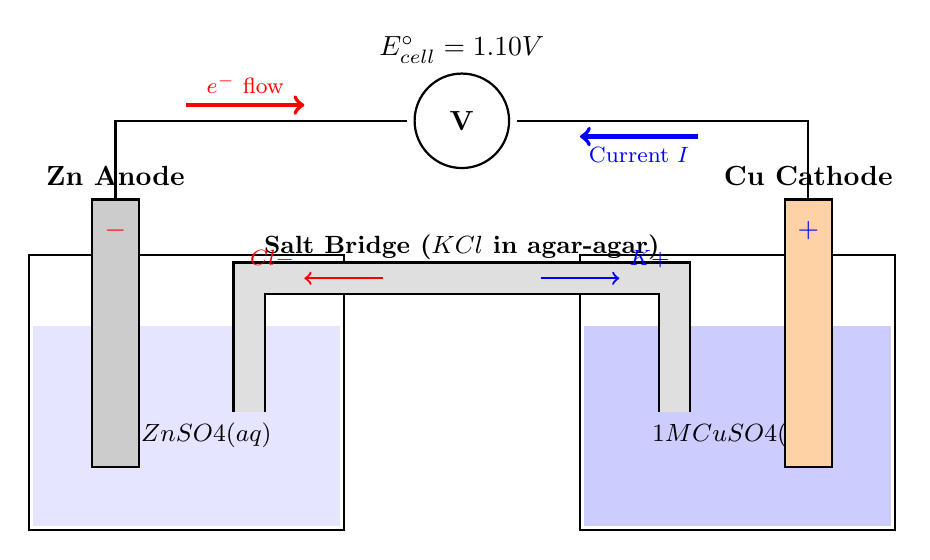
\begin{tikzpicture}[scale=1.0]
    % Anode beaker (Left)
    \draw[thick] (0,0) rectangle (4,3.5);
    \fill[blue!10] (0.05,0.05) rectangle (3.95,2.6);
    \node at (2,1.2) {\small $1\text{ M } \ce{ZnSO4(aq)}$};
    \draw[fill=gray!40, thick] (0.8,0.8) rectangle (1.4,4.2);
    \node at (1.1,4.5) {\textbf{Zn Anode}};
    \node[red, font=\bfseries] at (1.1,3.8) {$-$};
    
    % Cathode beaker (Right)
    \draw[thick] (7,0) rectangle (11,3.5);
    \fill[blue!20] (7.05,0.05) rectangle (10.95,2.6);
    \node at (9,1.2) {\small $1\text{ M } \ce{CuSO4(aq)}$};
    \draw[fill=orange!35, thick] (9.6,0.8) rectangle (10.2,4.2);
    \node at (9.9,4.5) {\textbf{Cu Cathode}};
    \node[blue, font=\bfseries] at (9.9,3.8) {$+$};

    % Salt Bridge
    \draw[line width=12pt, gray!25] (2.8,1.5) -- (2.8,3.2) -- (8.2,3.2) -- (8.2,1.5);
    \draw[thick] (2.6,1.5) -- (2.6,3.4) -- (8.4,3.4) -- (8.4,1.5);
    \draw[thick] (3.0,1.5) -- (3.0,3.0) -- (8.0,3.0) -- (8.0,1.5);
    \node at (5.5,3.6) {\small \textbf{Salt Bridge ($\ce{KCl}$ in agar-agar)}};
    
    % Salt bridge ions
    \draw[->, thick, red] (4.5,3.2) -- (3.5,3.2) node[above left] {\footnotesize $\ce{Cl-}$};
    \draw[->, thick, blue] (6.5,3.2) -- (7.5,3.2) node[above right] {\footnotesize $\ce{K+}$};

    % External circuit with Voltmeter
    \draw[thick] (1.1,4.2) -- (1.1,5.2) -- (4.8,5.2);
    \draw[thick] (6.2,5.2) -- (9.9,5.2) -- (9.9,4.2);
    \draw[fill=white, thick] (5.5,5.2) circle (0.6);
    \node at (5.5,5.2) {\textbf{V}};
    \node[above] at (5.5,5.8) {$E^\circ_{\text{cell}} = 1.10\text{ V}$};
    
    % Electron flow
    \draw[->, line width=1.5pt, red] (2.0,5.4) -- (3.5,5.4) node[midway, above] {\footnotesize $e^-$ flow};
    \draw[->, line width=1.5pt, blue] (8.5,5.0) -- (7.0,5.0) node[midway, below] {\footnotesize Current $I$};
\end{tikzpicture}
\caption{Schematic diagram of the Daniell Galvanic Cell.}
\label{fig:daniell_cell}
\end{figure}

\subsection{IUPAC Cell Representation Rules}
\begin{enumerate}[leftmargin=*]
    \item The \textbf{Anode} (electrode where oxidation occurs) is always placed on the \textbf{LEFT}.
    \item The \textbf{Cathode} (electrode where reduction occurs) is always placed on the \textbf{RIGHT}.
    \item A single vertical line ($|$) indicates a phase boundary between an electrode and solution.
    \item A double vertical line ($||$) indicates a salt bridge or porous partition connecting two half-cells with elimination of liquid junction potential.
    \item The Daniell cell is represented according to IUPAC notation as:
    \begin{equation}
        \ce{Zn(s) | Zn^2+(aq, } 1\text{ M)} \parallel \ce{Cu^2+(aq, } 1\text{ M) | Cu(s)}
    \end{equation}
    \item The \textbf{LOAN} mnemonic:
    \begin{center}
    \textbf{L}eft \quad $\bullet$ \quad \textbf{O}xidation \quad $\bullet$ \quad \textbf{A}node \quad $\bullet$ \quad \textbf{N}egative
    \end{center}
\end{enumerate}

\subsection{Functions \& Chemistry of the Salt Bridge}
A salt bridge is a U-shaped glass tube packed with a concentrated solution of an inert electrolyte ($\ce{KCl}, \ce{KNO3}, \ce{NH4NO3}$) solidified in a gelatinous agar-agar matrix.

\begin{conceptbox}[Four Indispensable Functions of the Salt Bridge]
\begin{enumerate}[leftmargin=*]
    \item \textbf{Completes the Electrical Circuit:} Provides an internal electrolytic conduction path allowing ions to migrate between compartments.
    \item \textbf{Maintains Electrical Neutrality:} 
    \begin{itemize}
        \item At the anode, $\ce{Zn^2+}$ ions continuously accumulate, creating a positive charge buildup that would immediately halt further electron release. Anions from the salt bridge ($\ce{Cl-}$) migrate into the anode beaker to neutralize excess $\ce{Zn^2+}$.
        \item At the cathode, $\ce{Cu^2+}$ ions are continuously discharged, leaving unneutralized $\ce{SO4^2-}$ anions. Cations from the salt bridge ($\ce{K+}$) migrate into the cathode beaker to neutralize excess $\ce{SO4^2-}$.
    \end{itemize}
    \item \textbf{Eliminates Liquid Junction Potential ($E_{lj} \approx 0$):} 
    When two dissimilar electrolyte solutions are in direct physical contact, ions diffuse across the boundary at different speeds, creating an unwanted boundary potential difference ($E_{lj}$). The salt bridge interposes an inert electrolyte with nearly equal cation and anion mobilities, eliminating $E_{lj}$.
    \item \textbf{Prevents Intermixing of Electrolytes:} Prevents bulk chemical precipitation reactions (e.g., direct spontaneous displacement of $\ce{Cu^2+}$ by $\ce{Zn}$ in bulk liquid).
\end{enumerate}
\end{conceptbox}

\begin{conceptbox}[Critical Criteria for Electrolyte in Salt Bridge]
\begin{enumerate}[leftmargin=*]
    \item \textbf{Equal Ionic Mobilities (Criterion of Equal Transference):}
    The transport numbers of the cation and anion must be virtually identical ($u_+ \approx u_-$):
    \begin{equation}
        t_+ \approx t_- \approx 0.50 \quad (\text{e.g., for } \ce{KCl}, t_{\ce{K+}} = 0.49, t_{\ce{Cl-}} = 0.51)
    \end{equation}
    Consequently, diffusion potential at the anode junction is exactly cancelled by the diffusion potential at the cathode junction.
    \item \textbf{Chemical Inertness:} The electrolyte must not undergo chemical or precipitation reactions with any component of the cell.
    \item \textbf{Prohibited Scenarios for $\ce{KCl}$:}
    A $\ce{KCl}$ salt bridge \textbf{cannot} be used if either half-cell contains ions of sparingly soluble chlorides:
    \begin{equation}
        \ce{Ag+}, \ce{Pb^2+}, \ce{Hg2^2+}, \ce{Tl+}
    \end{equation}
    because $\ce{AgCl}, \ce{PbCl2}, \ce{Hg2Cl2}$ precipitate out inside the pores of the agar gel, clogging the bridge and breaking electrical contact. For these cells, a $\ce{KNO3}$ or $\ce{NH4NO3}$ salt bridge must be employed.
\end{enumerate}
\end{conceptbox}

---

\section{The Electrochemical Series}

When elements are arranged in increasing order of their standard reduction potentials ($E^\circ_{\text{red}}$) at $298.15\text{ K}$, the resulting sequence is the \textbf{Electrochemical (Electromotive) Series}:

\begin{table}[htbp]
\centering
\small
\renewcommand{\arraystretch}{1.25}
\begin{tabularx}{\textwidth}{l X c p{4.2cm}}
\toprule
\textbf{Element} & \textbf{Standard Reduction Half-Reaction} & \textbf{$E^\circ_{\text{red}}$ (Volts)} & \textbf{Chemical Character / Reactivity} \\
\midrule
$\ce{Li}$ & $\ce{Li+ + e^- <=> Li(s)}$ & $-3.05$ & \textbf{Strongest Reducing Agent} in water \\
$\ce{K}$ & $\ce{K+ + e^- <=> K(s)}$ & $-2.93$ & Highly electropositive; reacts with water \\
$\ce{Ba}$ & $\ce{Ba^2+ + 2e^- <=> Ba(s)}$ & $-2.90$ & Rapidly displaces $\ce{H2}$ from cold water \\
$\ce{Ca}$ & $\ce{Ca^2+ + 2e^- <=> Ca(s)}$ & $-2.87$ & Strongly electropositive \\
$\ce{Na}$ & $\ce{Na+ + e^- <=> Na(s)}$ & $-2.71$ & Vigorous reaction with water \\
$\ce{Mg}$ & $\ce{Mg^2+ + 2e^- <=> Mg(s)}$ & $-2.37$ & Displaces $\ce{H2}$ from boiling water/steam \\
$\ce{Al}$ & $\ce{Al^3+ + 3e^- <=> Al(s)}$ & $-1.66$ & Displaces $\ce{H2}$ from dilute acids \\
$\ce{Zn}$ & $\ce{Zn^2+ + 2e^- <=> Zn(s)}$ & $-0.76$ & Typical laboratory $\ce{H2}$ generator \\
$\ce{Cr}$ & $\ce{Cr^3+ + 3e^- <=> Cr(s)}$ & $-0.74$ & Readily oxidized by $\ce{H+}$ \\
$\ce{Fe}$ & $\ce{Fe^2+ + 2e^- <=> Fe(s)}$ & $-0.44$ & Readily rusts; displaces $\ce{H2}$ from acids \\
$\ce{Cd}$ & $\ce{Cd^2+ + 2e^- <=> Cd(s)}$ & $-0.40$ & Moderately active metal \\
$\ce{Co}$ & $\ce{Co^2+ + 2e^- <=> Co(s)}$ & $-0.28$ & Displaces $\ce{H2}$ from acids slowly \\
$\ce{Ni}$ & $\ce{Ni^2+ + 2e^- <=> Ni(s)}$ & $-0.25$ & Passive in concentrated nitric acid \\
$\ce{Sn}$ & $\ce{Sn^2+ + 2e^- <=> Sn(s)}$ & $-0.14$ & Weak reducing agent \\
$\ce{Pb}$ & $\ce{Pb^2+ + 2e^- <=> Pb(s)}$ & $-0.13$ & Weak acid reaction (surface passivation) \\
\midrule
\textbf{$\ce{H2}$} & \textbf{$\ce{2H+ + 2e^- <=> H2(g)}$} & \textbf{$0.00$} & \textbf{Arbitrary Standard Reference (SHE)} \\
\midrule
$\ce{Cu}$ & $\ce{Cu^2+ + 2e^- <=> Cu(s)}$ & $+0.34$ & Unreactive toward dilute non-oxidizing acids \\
$\ce{I2}$ & $\ce{I2(s) + 2e^- <=> 2I^-}$ & $+0.54$ & Mild oxidizing agent \\
$\ce{Fe}$ & $\ce{Fe^3+ + e^- <=> Fe^2+}$ & $+0.77$ & Stable redox couple \\
$\ce{Hg}$ & $\ce{Hg2^2+ + 2e^- <=> 2Hg(l)}$ & $+0.79$ & Noble metal; dissolved only by oxidizing acids \\
$\ce{Ag}$ & $\ce{Ag+ + e^- <=> Ag(s)}$ & $+0.80$ & Noble metal; easily reduced \\
$\ce{Br2}$ & $\ce{Br2(l) + 2e^- <=> 2Br^-}$ & $+1.09$ & Strong oxidizing agent \\
$\ce{Cr2O7^2-}$ & $\ce{Cr2O7^2- + 14H+ + 6e^- <=> 2Cr^3+ + 7H2O}$ & $+1.33$ & Powerful analytical oxidant \\
$\ce{Cl2}$ & $\ce{Cl2(g) + 2e^- <=> 2Cl^-}$ & $+1.36$ & Powerful gaseous oxidant \\
$\ce{Au}$ & $\ce{Au^3+ + 3e^- <=> Au(s)}$ & $+1.50$ & Very noble; dissolved only by aqua regia \\
$\ce{MnO4-}$ & $\ce{MnO4^- + 8H+ + 5e^- <=> Mn^2+ + 4H2O}$ & $+1.51$ & Classic laboratory self-indicating oxidant \\
$\ce{F2}$ & $\ce{F2(g) + 2e^- <=> 2F^-}$ & $+2.87$ & \textbf{Strongest Oxidizing Agent} in chemistry \\
\bottomrule
\end{tabularx}
\caption{The Standard Electrochemical Series at $298.15\text{ K}$.}
\label{tab:electrochemical_series}
\end{table}

\subsection{Major Applications of the Electrochemical Series}

\subsubsection{1. Predicting Relative Oxidizing and Reducing Strengths}
\begin{itemize}[leftmargin=*]
    \item Species with the \textbf{most negative $E^\circ$} have the greatest tendency to lose electrons (undergo oxidation). Hence, metallic lithium ($\ce{Li}$) is the strongest reducing agent in aqueous solution.
    \item Species with the \textbf{most positive $E^\circ$} have the greatest tendency to accept electrons (undergo reduction). Hence, fluorine gas ($\ce{F2}$) is the strongest oxidizing agent.
\end{itemize}

\begin{atkinsbox}[Atkins Insight: Why is Lithium the Strongest Reducing Agent in Water?]
Although the ionization enthalpy of $\ce{Li(g)}$ is higher than that of $\ce{Na(g)}$ or $\ce{K(g)}$, the standard reduction potential of $\ce{Li+/Li}$ is by far the most negative ($-3.05\text{ V}$). This is explained by the Born-Haber thermodynamic cycle:
\begin{equation}
    \Delta H^\circ_{\text{oxidation}} = \Delta H^\circ_{\text{sub}} + \text{IE}_1 + \Delta H^\circ_{\text{hyd}}(\ce{Li+})
\end{equation}
Because the lithium cation $\ce{Li+}$ has an exceptionally small ionic radius ($r = 76\text{ pm}$), it possesses a colossal charge density, releasing an extraordinarily large hydration enthalpy ($\Delta H^\circ_{\text{hyd}} = -519\text{ kJ}\cdot\text{mol}^{-1}$) upon hydration:
\begin{equation}
    |\Delta H^\circ_{\text{hyd}}(\ce{Li+})| \gg |\Delta H^\circ_{\text{hyd}}(\ce{Na+})|
\end{equation}
This massive hydration energy completely offsets the high ionization enthalpy, driving $\Delta G^\circ$ for oxidation to an exceptionally negative value, making lithium the thermodynamically supreme reducing agent in water.
\end{atkinsbox}

\subsubsection{2. Spontaneity and Direction of Redox Reactions}
For any proposed cell reaction:
\begin{equation}
    E^\circ_{\text{cell}} = E^\circ_{\text{cathode}} - E^\circ_{\text{anode}} = E^\circ_{\text{Right}} - E^\circ_{\text{Left}}
\end{equation}
\begin{equation}
    \Delta G^\circ = -n F E^\circ_{\text{cell}}
\end{equation}
\begin{itemize}[leftmargin=*]
    \item If $E^\circ_{\text{cell}} > 0 \implies \Delta G^\circ < 0$: The cell reaction is thermodynamically \textbf{spontaneous} in the forward direction.
    \item If $E^\circ_{\text{cell}} < 0 \implies \Delta G^\circ > 0$: The cell reaction is \textbf{non-spontaneous} in the forward direction (spontaneous in the reverse direction).
    \item If $E^\circ_{\text{cell}} = 0 \implies \Delta G^\circ = 0$: The system is at \textbf{equilibrium}.
\end{itemize}

\subsubsection{3. Feasibility of Metal Displacement Reactions}
A metal with a \textbf{lower (more negative) $E^\circ_{\text{red}}$} will displace any metal with a \textbf{higher (more positive) $E^\circ_{\text{red}}$} from its aqueous salt solution:
\begin{equation}
    \ce{Zn(s) + Cu^2+(aq) -> Zn^2+(aq) + Cu(s)} \quad (E^\circ_{\text{cell}} = +1.10\text{ V} > 0, \text{ Spontaneous})
\end{equation}
Conversely, copper cannot displace zinc:
\begin{equation}
    \ce{Cu(s) + Zn^2+(aq) -> Cu^2+(aq) + Zn(s)} \quad (E^\circ_{\text{cell}} = -1.10\text{ V} < 0, \text{ Impossible})
\end{equation}

\subsubsection{4. Displacement of Hydrogen Gas from Non-Oxidizing Dilute Acids}
All metals positioned above hydrogen in the reduction potential series ($E^\circ_{\text{red}} < 0.00\text{ V}$) can reduce hydrogen ions from dilute acids ($\ce{HCl}, \text{dilute } \ce{H2SO4}$) to liberate $\ce{H2(g)}$:
\begin{equation}
    \ce{M(s) + z H+(aq) -> M^{z+}(aq) + \frac{z}{2} H2(g)} \quad \implies \quad E^\circ_{\text{cell}} = 0.00 - E^\circ_{\ce{M^{z+}/M}} > 0
\end{equation}
Metals below hydrogen ($E^\circ_{\text{red}} > 0.00\text{ V}$, such as $\ce{Cu}, \ce{Ag}, \ce{Au}, \ce{Hg}$) cannot displace $\ce{H2}$ gas from non-oxidizing acids.

\subsubsection{5. Thermal Stability of Metal Oxides}
Metals with high positive $E^\circ_{\text{red}}$ (noble metals like $\ce{Ag}, \ce{Au}, \ce{Hg}$) have very weak affinity for oxygen. Consequently, their oxides are thermally unstable and decompose into pure elemental metal and oxygen gas upon gentle heating:
\begin{equation}
    \ce{2Ag2O(s) ->[\Delta] 4Ag(s) + O2(g)} \qquad \ce{2HgO(s) ->[\Delta] 2Hg(l) + O2(g)}
\end{equation}
In contrast, oxides of metals with strongly negative $E^\circ$ ($\ce{Al2O3}, \ce{MgO}, \ce{CaO}$) are extremely stable and cannot be decomposed thermally.

---

\section{Comprehensive Master Solved Illustrations}

\begin{examplebox}[Coupled Metal--Insoluble Salt Electrode \& Solubility Product Calculation]
Given the standard reduction potentials at $298\text{ K}$:
\begin{align*}
    \ce{Ag+(aq) + e^- <=> Ag(s)} \quad & E^\circ = +0.799\text{ V} \\
    \ce{AgI(s) + e^- <=> Ag(s) + I^-(aq)} \quad & E^\circ = -0.151\text{ V}
\end{align*}
\begin{enumerate}[label=(\alph*)]
    \item Formulate a galvanic cell combining these two electrodes such that the cell reaction corresponds to the dissolution equilibrium of $\ce{AgI(s)}$.
    \item Calculate the standard cell EMF ($E^\circ_{\text{cell}}$).
    \item Evaluate the solubility product constant ($K_{sp}$) of $\ce{AgI}$ at $298\text{ K}$.
\end{enumerate}
\tcblower
\textbf{Part (a): Cell Formulation:}
We desire the net reaction to be the dissolution of $\ce{AgI}$:
\begin{equation*}
    \ce{AgI(s) <=> Ag+(aq) + I^-(aq)}
\end{equation*}
Subtracting the $\ce{Ag+/Ag}$ reduction reaction from the $\ce{AgI/Ag,I-}$ reduction reaction:
\begin{align*}
    \text{Cathode (Reduction):} \quad & \ce{AgI(s) + e^- -> Ag(s) + I^-(aq)} \quad & E^\circ = -0.151\text{ V} \\
    \text{Anode (Oxidation):} \quad & \ce{Ag(s) -> Ag+(aq) + e^-} \quad & E^\circ_{\text{ox}} = -0.799\text{ V} \\
    \hline
    \text{Overall Net Reaction:} \quad & \ce{AgI(s) <=> Ag+(aq) + I^-(aq)} &
\end{align*}
The cell is represented as:
\begin{equation*}
    \ce{Ag(s) | Ag+(aq)} \parallel \ce{I^-(aq) | AgI(s) | Ag(s)}
\end{equation*}

\textbf{Part (b): Standard Cell EMF ($E^\circ_{\text{cell}}$):}
\begin{equation*}
    E^\circ_{\text{cell}} = E^\circ_{\text{cathode}} - E^\circ_{\text{anode}} = (-0.151\text{ V}) - (+0.799\text{ V}) = -0.950\text{ V}
\end{equation*}

\textbf{Part (c): Solubility Product ($K_{sp}$):}
At equilibrium:
\begin{equation*}
    \Delta G^\circ = -n F E^\circ_{\text{cell}} = -RT \ln K_{sp}
\end{equation*}
\begin{equation*}
    \log K_{sp} = \frac{n E^\circ_{\text{cell}}}{0.0591} = \frac{1 \times (-0.950)}{0.0591} \approx -16.074
\end{equation*}
\begin{equation*}
    K_{sp} = 10^{-16.074} = 10^{0.926} \times 10^{-17} \approx 8.43 \times 10^{-17}\ \text{mol}^2\cdot\text{L}^{-2}
\end{equation*}
\end{examplebox}

\begin{examplebox}[Prediction of Disproportionation Reaction Feasibility]
Given the following standard electrode potentials in aqueous acidic solution:
\begin{align*}
    \ce{Cu^2+(aq) + e^- <=> Cu+(aq)} \quad & E^\circ_1 = +0.153\text{ V} \\
    \ce{Cu+(aq) + e^- <=> Cu(s)} \quad & E^\circ_2 = +0.518\text{ V}
\end{align*}
Determine whether cuprous ion ($\ce{Cu+}$) is stable in aqueous solution, or whether it spontaneously disproportionates into $\ce{Cu^2+}$ and $\ce{Cu(s)}$. Calculate the equilibrium constant ($K_c$) for the disproportionation reaction at $298\text{ K}$.
\tcblower
\textbf{Step 1: Write the Disproportionation Half-Reactions:}
\begin{align*}
    \text{Reduction:} \quad & \ce{Cu+(aq) + e^- -> Cu(s)} \quad & E^\circ_{\text{cathode}} = +0.518\text{ V} \\
    \text{Oxidation:} \quad & \ce{Cu+(aq) -> Cu^2+(aq) + e^-} \quad & E^\circ_{\text{anode}} = +0.153\text{ V} \\
    \hline
    \text{Net Reaction:} \quad & \ce{2Cu+(aq) <=> Cu^2+(aq) + Cu(s)} &
\end{align*}

\textbf{Step 2: Calculate $E^\circ_{\text{cell}}$:}
\begin{equation*}
    E^\circ_{\text{cell}} = E^\circ_{\text{cathode}} - E^\circ_{\text{anode}} = (+0.518\text{ V}) - (+0.153\text{ V}) = +0.365\text{ V}
\end{equation*}
Since $E^\circ_{\text{cell}} > 0$ ($\Delta G^\circ < 0$), the forward reaction is \textbf{thermodynamically highly spontaneous}. Thus, $\ce{Cu+}$ ions are unstable in aqueous solution and spontaneously \textbf{disproportionate} into $\ce{Cu^2+}$ and metallic copper.

\textbf{Step 3: Calculate the Equilibrium Constant ($K_c$):}
\begin{equation*}
    \log K_c = \frac{n E^\circ_{\text{cell}}}{0.0591} = \frac{1 \times 0.365}{0.0591} = 6.176
\end{equation*}
\begin{equation*}
    K_c = \frac{[\ce{Cu^2+}]}{[\ce{Cu+}]^2} = 10^{6.176} = 10^{0.176} \times 10^6 \approx 1.50 \times 10^6
\end{equation*}
The immense magnitude of $K_c$ ($1.5 \times 10^6$) proves that virtually all $\ce{Cu+}$ ions disproportionate in aqueous media unless stabilized by complexation (e.g., $[\ce{Cu(CN)2}]^-$) or precipitation (e.g., $\ce{CuCl(s)}$).
\end{examplebox}
